\documentclass[aspectratio=169]{beamer}
\usetheme{hogent}
\usecolortheme{hgwhite} % witte achtergrond, zwarte tekst

%% common.tex -- Code die in elk .tex-bestand terug komt

%% Packages

\usepackage[dutch]{babel}
\usepackage{graphicx}
\usepackage{comment,enumerate,hyperref}
\usepackage{amsmath,amsfonts,amssymb}
\usepackage{eurosym}
\usepackage{booktabs}
\usepackage{multicol,multirow}
\usepackage{listings}

\usepackage[outputdir=out]{minted}
%\usepackage{minted}

\usepackage[backend=biber,style=apa]{biblatex}
\DeclareLanguageMapping{dutch}{dutch-apa}

\usepackage{csquotes}

%% Variabelen, elk academiejaar aan te passen
\newcommand{\academicyear}{2023--2024 (revisie: \today)}
\newcommand{\lecturers}{Thomas Aelbrecht \and Thomas Parmentier \and Bert Van Vreckem}
\newcommand{\coursename}{Research Methods (IT)}

%% Macro's en commando's

%% \alertbox: een kader voor tekst die moet opvallen
\newcommand{\alertbox}[2][hgblue]{%
  \setbeamercolor{alertbox}{bg=#1,fg=white}
  \begin{beamercolorbox}[sep=2pt,center]{alertbox}
    \textbf{#2}
  \end{beamercolorbox}
}


\addbibresource{rm1-werken-met-latex.bib}

%---------- Info over de presentatie ------------------------------------------

\title{Module 1. Working with \LaTeX.}
\subtitle{Research Methods}
\author{\lecturers}   % Pas waarden aan in common.tex
\date{\academicyear}

\begin{document}

\begin{frame}
  \maketitle
\end{frame}

\begin{frame}
  \frametitle{Inhoud}

  \tableofcontents
\end{frame}

\section{Inleiding}

\subsection{Filosofie, geschiedenis}

\begin{frame}
  \frametitle{Filosofie: waarom {\LaTeX}?}

  \begin{itemize}
    \item<+-> WYSIWYG tekstverwerkers dwingen auteurs om de vormgeving te verzorgen.
    \item<+-> Gevolg is slechte, inconsistente opmaak van documenten.
    \item<+-> Goede vormgeving van teksten is een \textit{specialisatie}, en wordt best
    uit handen van auteurs genomen.
    \item<+-> {\LaTeX} zorgt dat auteurs enkel over de \textit{inhoud} en \textit{structuur} van de tekst moet nadenken.
  \end{itemize}
\end{frame}

\begin{frame}[plain]
  \frametitle{Geschiedenis}

  \begin{columns}[c]

    \column{.67\textwidth}
    \begin{itemize}
      \item<+-> 1977: Donald Knuth vindt de drukproeven van zijn boek \textit{The art of Computer Programming} afschuwelijk
      \item<+-> 1978: Schreef dan maar zelf een tekstzetsysteem, {\TeX}
      \item<+-> 1989: Versie 3.0, sindsdien enkel bugfix-releases (convergeren naar \(\pi\))
      \item<+-> 1980s: Leslie Lamport ontwikkelt markup-taal voor {\TeX}: {\LaTeX}
    \end{itemize}

    \column{.33\textwidth}
    \begin{center}
      \only<1-3>{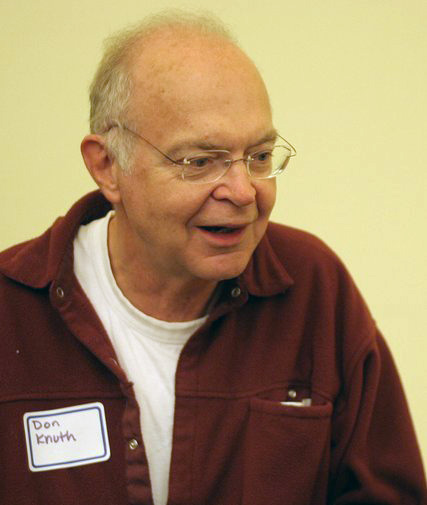
\includegraphics[width=\textwidth]{1/donald-knuth}}
      \only<4->{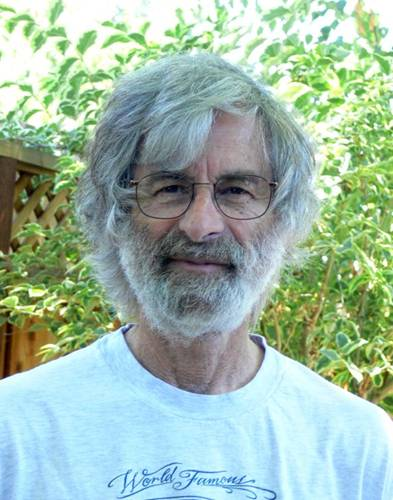
\includegraphics[width=\textwidth]{1/leslie-lamport}}
    \end{center}

  \end{columns}
\end{frame}

\subsection{Voorbeelden}

\begin{frame}
  \frametitle{Voorbeelden---papers}

  {\LaTeX} is de norm voor wetenschappelijke publicaties in computerwetenschappen, wiskunde, fysica, enz.

  \begin{center}
    
\includegraphics[height=.6\textheight]{1/latex-paper}
  \end{center}

\end{frame}

\begin{frame}
  \frametitle{Voorbeelden---boeken}

  Ook: cursussen, thesissen, enz.

  \begin{center}
    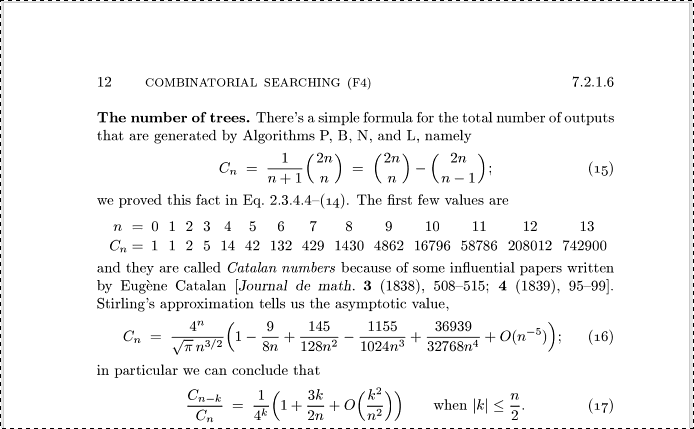
\includegraphics[height=.6\textheight]{1/latex-book}
  \end{center}

\end{frame}

\begin{frame}
  \frametitle{Voorbeelden---presentaties}

  \begin{center}
    vb.\ deze presentatie\ldots
  \end{center}

\end{frame}

\begin{frame}
  \frametitle{Voordelen}

  \begin{itemize}
    \item<+-> Enkel bezighouden met inhoud, goede en consistente opmaak gegarandeerd.
    \item<+-> Stijl aanpassen zonder inhoud te wijzigen.
    \item<+-> Tekstformaat \(\Rightarrow\) geschikt voor versiebeheersysteem!
    \item<+-> Is de norm in verschillende onderzoeksdomeinen, o.a.\ computerwetenschappen
  \end{itemize}
\end{frame}


\begin{frame}
  \frametitle{Nadelen}

  \begin{itemize}
    \item<+-> Zware leercurve \(\Rightarrow\) copy paste voorbeelden, gebruik infobronnen, vraag hulp
    \item<+-> Soms is gewenste opmaak niet makkelijk te bereiken (vb.~tabellen)
  \end{itemize}

  \uncover<1->{%
    \begin{center}
      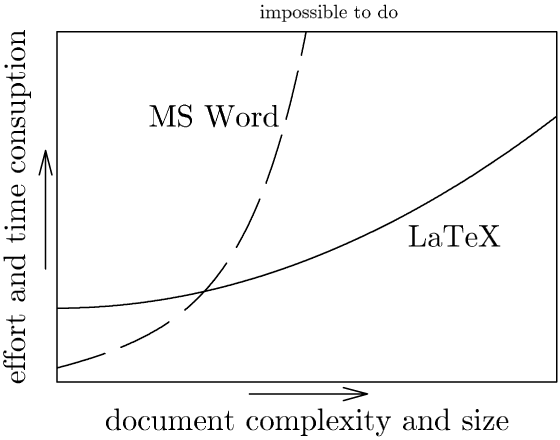
\includegraphics[height=.5\textheight]{1/word-vs-latex}
  \end{center}}
\end{frame}

\subsection{Hulp zoeken}

\begin{frame}
  \frametitle{Hulp zoeken}

  \begin{itemize}
    \item Tobias Oetiker, et al., \emph{The Not So Short Introduction to {\LaTeXe}}, 2011 (a.k.a. ``lshort'', versie 5.01)
    \item {\TeX} --- {\LaTeX} StackExchange (Q \& A site): \url{http://tex.stackexchange.com/}
    \item \emph{{\LaTeX} Wikibook}, \url{http://en.wikibooks.org/wiki/LaTeX}
    \item Handleidingen van packages (pdf)
  \end{itemize}

\end{frame}

\section{Aan de slag met {\LaTeX}}

\subsection{Documentstructuur}

\begin{frame}
  \frametitle{Werkwijze}

  \begin{itemize}
    \item<+-> Schrijf tekst in {\LaTeX}\\
    = tekstbestand! (markuptaal zoals HTML)
    \item<+-> Compileer (evt.\ verschillende keren)
    \item<+-> Bekijk resultaat in PDF
  \end{itemize}
\end{frame}

\begin{frame}[fragile]
  \frametitle{{\LaTeX} commando's}

  \begin{block}{Basis-syntax}
    \verb|\commandonaam[optionele,argumenten]{arg1}{arg2}|
  \end{block}

  \pause

  Bijvoorbeeld:

  \begin{itemize}
    \item<+-> \verb|\documentclass[a4paper,pdftex,12pt]{article}|
    \item<+-> \verb|\'{e}l\`{e}ve| \(\Rightarrow\) \'el\`eve
    \item<+-> \verb|\begin{itemize}|\\
    \verb|\item lijst|\\
    \verb|\end{itemize}|
  \end{itemize}

\end{frame}

\begin{frame}[fragile]
  \frametitle{Een document opbouwen}

  \begin{center}
    \alert{%
      \only<1>{Definitie documentsoort (hier: artikel)}
      \only<2>{``body'' van het document}
      \only<3>{Documentinhoud}
      \only<4>{Extra functionaliteit beschikbaar maken}
      \only<5>{Titel, auteur komt in ``preamble''}
      \only<6>{Titel in document invoegen}
    }
  \end{center}

  \begin{semiverbatim}
    \uncover<1->{\alert<1>{\\documentclass[a4paper,12pt]\{article\}}}
    \uncover<4->{\alert<4>{\\usepackage[dutch]\{babel\}}}
    \uncover<5->{\alert<5>{\\title\{Minimaal \{\\LaTeX\} document\}}}
    \uncover<5->{\alert<5>{\\author\{Bert \{Van Vreckem\}\}}}
    \uncover<5->{\alert<5>{\\date\{\\today\}}}
    \uncover<2->{\alert<2>{\\begin\{document\}}}
    \uncover<6->{\alert<6>{\\maketitle}}
    \uncover<3->{\alert<3>{Lorem ipsum dolor sit amet, consectetur adipiscing elit.}}
    \uncover<2->{\alert<2>{\\end\{document\}}}
  \end{semiverbatim}

\end{frame}

\begin{frame}
  \frametitle{Resultaat}

  \begin{center}
    
\includegraphics[height=.6\textheight]{1/minimaal-document}
  \end{center}
\end{frame}

\begin{frame}[fragile]
  \frametitle{Documenttypes}

  \begin{center}
    \begin{semiverbatim}
      \\documentclass[\alert<2>{OPTIONS}]\{\alert<1>{TYPE}\}
    \end{semiverbatim}
  \end{center}

  \only<1>{%
    \begin{center}
      \begin{tabular}{ll}
        \toprule
        TYPE & soort document \\
        \midrule
        \texttt{article} & artikel, paper, korte tekst \\
        \texttt{beamer} & presentatie \\
        \texttt{book} & boek \\
        \texttt{report} & (lang) rapport, thesis, verslag, \ldots \\
      \end{tabular}
    \end{center}
  }
  \only<2>{%
    \begin{center}
      \begin{tabular}{ll}
        \toprule
        OPTION & soort document \\
        \midrule
        \texttt{12pt} & 12-puntsletters (ipv 10pt) \\
        \texttt{a4paper} & A4 (ipv Am. Letter) \\
        \texttt{twocolumn} & gebruikelijk bij artikels \\
        \texttt{twoside} & voor dubbelzijdig afdrukken \\
      \end{tabular}
    \end{center}
  }
\end{frame}

\begin{frame}[fragile]
  \frametitle{Documentstructuur}

  \begin{center}
    \begin{tabular}{ll}
      \verb?\part? & (geen invloed op hoofdstuknummers) \\
      \verb?\chapter? & (enkel in \texttt{book}, \texttt{report}) \\
      \verb?\section? & \\
      \verb?\subsection? & \\
      \verb?\subsubsection? & (niet in \texttt{book}, \texttt{report}) \\
      \verb?\paragraph? & \\
      \verb?\subparagraph? & \\
      &\\
      \verb?\appendix? & vanaf hier wordt \verb?\chapter? een Bijlage \\
      \verb?\label{?\texttt{\ldots}\verb?}? & voor verwijzingen (met \verb|\ref{LABEL}|)
    \end{tabular}
  \end{center}
\end{frame}

\begin{frame}[fragile]
  \frametitle{Preamble---Nuttige packages}

  \begin{description}
    \item[\texttt{\textbackslash{}usepackage\{amsfonts\}}] AMS math packages: extra wiskundige
    \item[\texttt{\textbackslash{}usepackage\{amsmath\}}] symbolen (o.a.\ getallenverzamelingen
    \item[\texttt{\textbackslash{}usepackage\{amssymb\}}] \(\mathbb{N}, \mathbb{R}, \mathbb{Z}, \mathbb{Q}\), etc.)
    \pause
    \item[\texttt{\textbackslash{}usepackage[dutch]\{babel\}}] Taalinstellingen: woordsplitsingen, commando's voor speciale karakters (``dutch'' voor NL)
    \pause
    \item[\texttt{\textbackslash{}usepackage\{eurosym\}}] Euro-symbool (\euro)
    \pause
    \item[\texttt{\textbackslash{}usepackage\{fancyhdr\}}] Pagina-opmaak met hoofd- en voettekst
    \pause
    \item[\texttt{\textbackslash{}usepackage\{graphicx\}}] Invoegen van figuren
  \end{description}
\end{frame}

\begin{frame}[fragile]
  \frametitle{Preamble---Nuttige packages}

  \begin{description}
    \item[\texttt{\textbackslash{}usepackage[pdftex,bookmarks=true]\{hyperref\}}] PDF krijgt klikbare links \& verwijzingen, inhoudstafel \pause
    \item[\texttt{\textbackslash{}usepackage[utf8]\{inputenc\}}] Accenten gebruiken in tekst (vb. é ipv \verb|\'e|) \pause
    \item[\texttt{\textbackslash{}usepackage\{listings\}}] Broncode mooi opmaken \pause
    \item[\texttt{\textbackslash{}usepackage\{multirow\}}] Tekst over verschillende cellen in tabellen \pause
    \item[\texttt{\textbackslash{}usepackage\{rotating\}}] Tabellen en figuren roteren \pause
    \item[\texttt{\textbackslash{}usepackage\{lipsum\}}] Vultekst (lorem ipsum dolor sit amet\ldots)
  \end{description}
\end{frame}

\subsection{Tekst schrijven}

\begin{frame}[fragile]
 \frametitle{Tekstopmaak}

 \begin{itemize}
   \item<+-> Speciale tekens ({\LaTeX} syntax): \% \$ \& \{ \} \textbackslash{} enz: \\
   \begin{semiverbatim}
     \\\% \\\$ \\\& \\\{ \\\} \\textbackslash\{\}
   \end{semiverbatim}
   \item<+-> Ligaturen: \textrm{fi fl ffi ffl} (automatisch opgemaakt)
   \item<+-> Accenten: \'{e} \`{e} \^{e} \"{e} \={e} \c{c} enz.
   \begin{semiverbatim}
     \\'\{e\} \\`\{e\} \\^\{e\} \\"\{e\} \\=\{e\} \\c\{c\} enz.
   \end{semiverbatim}
   \item<+-> Ellipsis (\ldots): \texttt{\textbackslash{}ldots}
   \item<+-> Aanhalingstekens: `enkel' ``dubbel''
   \begin{verbatim}
   `enkel' ``dubbel''
   \end{verbatim}
 \end{itemize}
\end{frame}

\begin{frame}[fragile]
 \frametitle{Letterstijlen}

 \begin{center}
   \begin{tabular}{ll}
     \toprule
     Commando & resultaat \\
     \midrule
     \verb?\emph{xxx}?   & \emph{Benadrukken} (\textrm{\emph{cursief}} of \textsf{\emph{`slanted'}})\\
     \verb?\textit{xxx}? & \textit{Cursieve tekst} \\
     \verb?\textbf{xxx}? & \textbf{Vetgedrukte tekst} \\
     \verb?\texttt{xxx}? & \texttt{Monogespatieerde letters} \\
     \verb?\textrm{xxx}? & \textrm{Schreefletters}  \\
     \verb?\textsf{xxx}? & \textsf{Schreefloze letters}  \\
     \verb?\textsc{xxx}? & \textsc{Small Caps} \\
   \end{tabular}
 \end{center}

\end{frame}

\begin{frame}[fragile]
 \frametitle{Lijstomgevingen}

 \begin{columns}[c]
   \column{.49\textwidth}
   \begin{verbatim}
   \begin{itemize}
   \item Een onderdeel
   \item Nog een onderdeel
   \end{itemize}
   \end{verbatim}

   \column{.49\textwidth}
   \begin{itemize}
     \item Een onderdeel
     \item Nog een onderdeel
   \end{itemize}
 \end{columns}

 \pause

 \begin{columns}[c]
   \column{.49\textwidth}
   \begin{verbatim}
   \begin{enumerate}
   \item Een onderdeel
     \begin{enumerate}
     \item extra niveau
     \end{enumerate}
   \item Nog een onderdeel
   \end{enumerate}
   \end{verbatim}

   \column{.49\textwidth}
   \begin{enumerate}
     \item Een onderdeel
     \begin{enumerate}
       \item extra niveau
     \end{enumerate}
     \item Nog een onderdeel
   \end{enumerate}
 \end{columns}

\end{frame}

\section{Figuren, tabellen, enz.\ invoegen}

\subsection{Figuren}

\begin{frame}[fragile,plain]
 \frametitle{Figuren invoegen}

 \begin{columns}[c]
   \column{.65\textwidth}

\begin{semiverbatim}
\alert<1>{\\begin\{figure\}}
\alert<2>{\\includegraphics[width=\\textwidth]
 \{1/donald-knuth\}}
\alert<3>{\\caption\{\alert<4>{\\label\{fig:don\}}Donald Knuth, auteur van
 \{\\TeX\}\}}
\alert<1>{\\end\{figure\}}
\end{semiverbatim}

   \column{.35\textwidth}
   \begin{figure}
     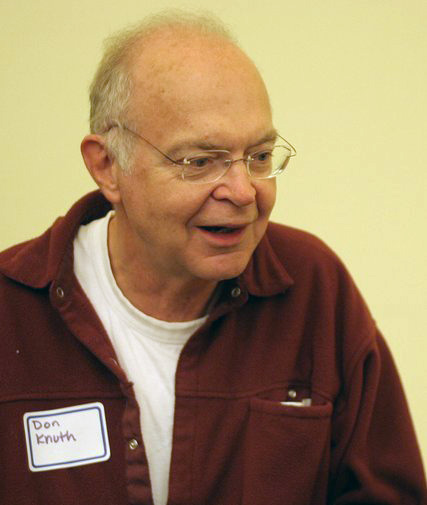
\includegraphics[width=\textwidth]{1/donald-knuth}
     \caption{\label{fig:don}Donald Knuth, auteur van {\TeX}}
   \end{figure}

 \end{columns}

\end{frame}

\subsection{Tabellen}

\begin{frame}[fragile]
 \frametitle{Tabellen invoegen}

 \begin{columns}[c]
   \column{.6\textwidth}
   \small
\begin{semiverbatim}
\alert<1>{\\begin\{table\}}
\alert<3>{\\begin\{tabular\}\{\alert<4>{l||c|r}\}}
\alert<4>{\\hline}
cel11 \alert<5>{&}
\alert<7>{\\multicolumn\{2\}\{c\}\{cel12\}} \alert<6>{\\\\}
\alert<4>{\\hline \\hline}
cel21 \alert<5>{&} cel22 \alert<5>{&}
\alert<7>{\\multirow\{2\}\{*\}\{cel23\}} \alert<6>{\\\\}
cel31 \alert<5>{&} cel32 \alert<5>{&} \alert<6>{\\\\}
\alert<3>{\\end\{tabular\}}
\alert<2>{\\caption\{Een voorbeeldje van
 wat je met tabellen kan doen\}
 \\label\{tab:vb_tabel\}}
\alert<1>{\\end\{table\}}
\end{semiverbatim}

   \column{.4\textwidth}
   \begin{table}
     \begin{tabular}{l||c|r}
       \hline
       cel11 & \multicolumn{2}{c}{cel12} \\
       \hline \hline
       cel21 & cel22 & \multirow{2}{*}{cel23} \\
       cel31 & cel32 & \\
     \end{tabular}
     \caption{Een voorbeeldje van wat je met tabellen kan doen}
     \label{tab:vb_tabel}
   \end{table}

 \end{columns}
\end{frame}

\subsection{Broncode}

\begin{frame}[fragile]
 \frametitle{Broncode invoegen}
 \framesubtitle{Eenvoudigste vorm: \texttt{verbatim}}

\begin{semiverbatim}
\alert{\\begin\{verbatim\}}
public class MyApp \{
 public static void main(String args[]) \{
   System.out.println("Hello World");
 \}
\}
\alert{\\end\{verbatim\}}
\end{semiverbatim}

 \(\Rightarrow\)

\begin{verbatim}
public class MyApp {
 public static void main(String args[]) {
   System.out.println("Hello World");
 }
}
\end{verbatim}

\end{frame}

\begin{frame}[fragile]
 \frametitle{Broncode invoegen}
 \framesubtitle{\texttt{listings} package}

\begin{semiverbatim}
\\lstset\{\%
language=java,  breaklines=true,  numbers=left,
frame=single, caption=\{Mijn eerste Java-programma.\},
label=code:helloworld\}

\alert{\\begin\{lstlisting\}}
public class MyApp \{
 public static void main(String args[]) \{
   System.out.println("Hello World");
 \}
\}
\alert{\\end\{lstlisting\}}
\end{semiverbatim}

\end{frame}

\begin{frame}[fragile]
  \frametitle{Broncode invoegen}
  \framesubtitle{\texttt{listings} package}

  \lstset{%
    language=java,    breaklines=true,
    numbers=left,     frame=single,
    caption={Mijn eerste Java-programma.},
    label=code:helloworld,
    gobble=2
  }

  \begin{lstlisting}
  public class MyApp {
    public static void main(String args[]) {
      System.out.println("Hello World");
    }
  }
  \end{lstlisting}

\end{frame}

\begin{frame}[fragile]
  \frametitle{Broncode invoegen}
  \framesubtitle{\texttt{minted} package}

  \begin{semiverbatim}
  \\setminted\{%
    bgcolor=gray!20,gobble=2, linenos,
    numbers=left,frame=single\}

  \\begin\{minted\}\{java\}
    public class MyApp \{
      public static void main(String args[]) \{
        System.out.println("Hello World");
      \}
    \}
  \\end\{minted\}
  \end{semiverbatim}
\end{frame}


\begin{frame}[fragile]
  \frametitle{Broncode invoegen}
  \framesubtitle{\texttt{minted} package}
  \setminted{bgcolor=gray!20,gobble=4,linenos,numbers=left,frame=single}
  \begin{minted}{java}
    public class MyApp {
      public static void main(String args[]) {
        System.out.println("Hello World");
      }
    }
  \end{minted}
\end{frame}

\subsection{Literatuurlijst}

\begin{frame}[fragile]
  \frametitle{Literatuurlijst}

  \begin{itemize}
    \item<+-> Literatuurlijst is belangrijk onderdeel van een eindwerk
    \item<+-> Strakke regels voor opmaak (HOGENT: APA-stijl)
    \item<+-> {\LaTeX}, meer bepaald Bib{\LaTeX} helpt:
    \begin{itemize}
      \item<+-> ``bibliografische databank'' (in tekstformaat)
      \item<+-> Automatisch correcte opmaak
      \item<+-> Verwijzingen vanuit uit de tekst (\verb|\textcite{}|)
      \item<+-> Ondersteuning via externe tools (e.g. JabRef, Mendeley Desktop)
    \end{itemize}
  \end{itemize}

  \pause Zie vervolg cursus!
\end{frame}

\section{Tot slot}

\begin{frame}[fragile]
 \frametitle{Tot slot}

  Een heleboel niet besproken!

  \begin{itemize}
    \item<+-> Wiskundige formules, vb.
    \begin{semiverbatim}
      \$x=-\\frac\{b \\pm \\sqrt\{b\^{}2 - 4ac\}\}\{2a\}\$
    \end{semiverbatim}
    \(x=-\frac{b \pm \sqrt{b^2 - 4ac}}{2a}\)
    \item<+-> Honderden packages (RTFM, Google is your friend)
    \item<+-> Presentaties met Beamer (baseer je bv.\ op het sjabloon op \url{https://github.com/HoGentTIN/presentatie-latex-sjabloon})

  \end{itemize}
\end{frame}

\end{document}
